\chapter{Projecto - Parte 2}\label{ch:projeto-parte2}

Nesta fase do projeto, o objetivo foi criar um sistema autónomo inteligente capaz de se movimentar num espaço com dimensões fixas onde existem obstáculos e alvos.
A finalidade do agente prospetor é recolher os alvos e evitar os obstáculos presentes no ambiente (ver figura~\ref{fig:agente-prospetor}).

\begin{figure}[H]
    \label{fig:agente-prospetor}
    \begin{center}
        \resizebox{100mm}{!}{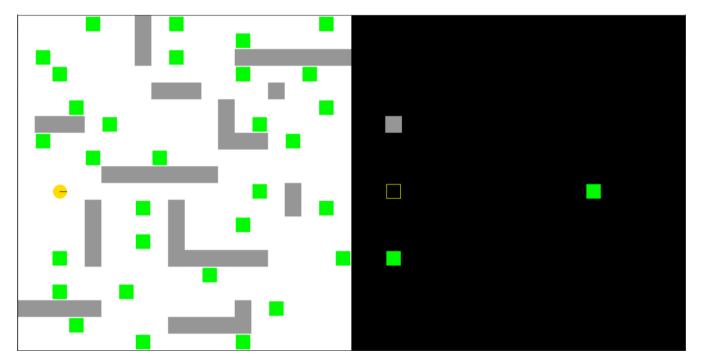
\includegraphics{../figures/agente-prospetor}}
    \end{center}
    \caption{Representação visual desta fase do projeto.}
\end{figure}

\section{Agentes Reativos}\label{sec:agentes-reativos}

Na secção da arquitetura de agentes (ver secção~\ref{sec:arquiteturas-agente}), foi referido que uma arquitetura reativa é caracterizada pela associação direta entre a perceções e ações.

Inerente a esta arquitetura, está o conceito de mecanismo de reação.
Este mecanismo apresenta os seguintes componentes:

\begin{itemize}
    \item \textbf{Estímulo}: Define a informação que é extraída de uma percepção, de forma a ser utilizada na ativação de uma resposta.
    Vários estímulos podem ser ativados por uma única perceção.
    Estão regularmente associados a um parâmetro de intensidade.
    \item \textbf{Resposta}: Representa a geração de uma resposta a estímulos, inerentemente ligada a uma ação a ser executada e à sua respetiva prioridade.
    Além de poder ser ativada por um estímulo, uma resposta pode ser ativada diretamente por uma percepção, de forma a garantir restrições de ativação (guardas) se necessário.
    \item \textbf{Reação}: Associa estímulos a respostas.
\end{itemize}

Um agente reativo é composto por um conjunto de reações, que devem ser organizadas de forma modular em módulos comportamentais designados por comportamentos.
Isto permite as reações internas do agente sejam encapsuladas, facilitando a sua manutenção e escalabilidade.

Um comportamento (ver figura~\ref{fig:agente-reativo-comportamento}) define um módulo comportamental associado a um agente reativo. Encapsula um conjunto de reações relacionadas entre si, possivelmente com uma sequência temporal, de forma a atingir um ou ou mais objetivos (e.g., evitar obstáculos, recolher alvos, etc). Associado a um objetivo podem existir sub-objetivos.

\begin{figure}[H]
    \label{fig:agente-reativo-comportamento}
    \begin{center}
        \resizebox{100mm}{!}{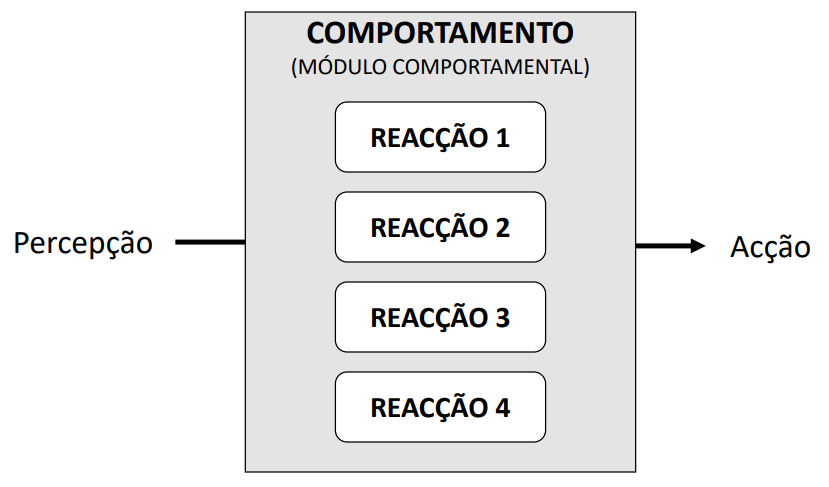
\includegraphics{../figures/agente-reativo-comportamento}}
    \end{center}
    \caption{Módulo comportamental de um agente reativo.
    Retirado de~\cite{isel:iasa:slides:arq-agentes-reativos-parte-1}.}
\end{figure}

Tipos de Comportamento:

\begin{itemize}
    \item \textbf{Comportamento Fixo}: Caracterizado por ter uma resposta fixa, pois gera uma ação em permanência;
    \item \textbf{Comportamento Simples}: Reação;
    \item \textbf{Comportamento Composto}: Agrega sub-comportamentos, ao qual está associado um mecanismo de seleção de ação de forma a determinar a ação a realizar em função das respostas dos mesmos).
\end{itemize}

Visto que, em comportamentos compostos, uma perceção pode ativar várias múltiplas reacções, as quais geram diferentes ações, é necessário definir mecanismos aos quais estão associados políticas de seleção de ação:

%\begin{itemize}
    TODO

\section{Biblioteca ECR}\label{sec:biblioteca-ecr}

TODO
